\subsection{DeadBindingRemoval.fs}
Following the instructions in the lecture slides\footnote{Lecture slides, 9-Optim-Fasto.pdf} dead binding elimination has been implemented. In the case of \textit{Var} we know there will not be any IO, and we can not optimize the abstract syntax tree. Thus we construct a triple tuple of \textit{false} for IO, an empty symbol table with the variable name appended and 'Var (name, pos)'. (lines 63 - 70 of DeadBindingRemoval.fs).\\
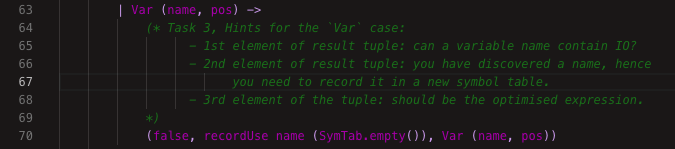
\includegraphics[width=\linewidth]{Materials/Optimization/VarDBE}\\
For \textit{Index} we recursively optimize the expression and return the results thereof. (lines 72 - 79).\\
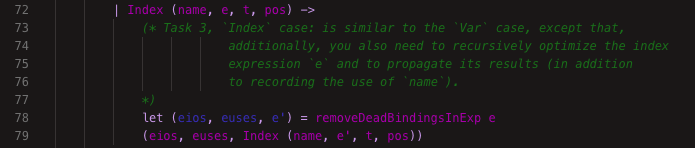
\includegraphics[width=\linewidth]{Materials/Optimization/IndexDBE}\\
For \textit{Let} we recursively optimize the body and the expression. We now optimize based on whether we can remove the expression or not. (lines 81 - 102).\\
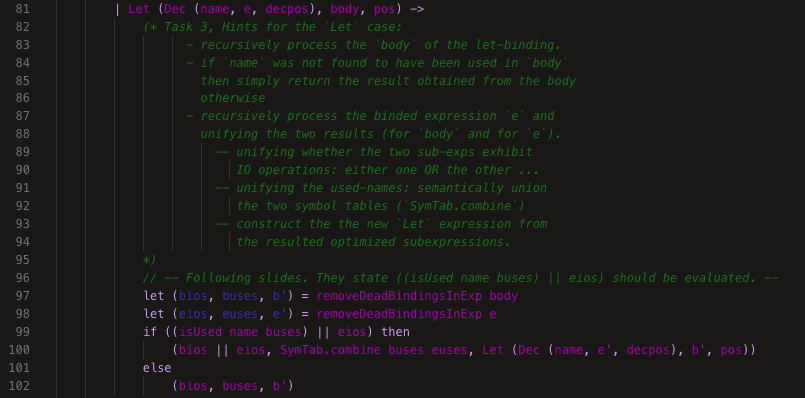
\includegraphics[width=\linewidth]{Materials/Optimization/LetDBE}\\
Dead binding elimination is done similarly for all other expressions.
